\normalem
\section{Background}
\lipsum[2-4] \\


\begin{figure}
    \centering
    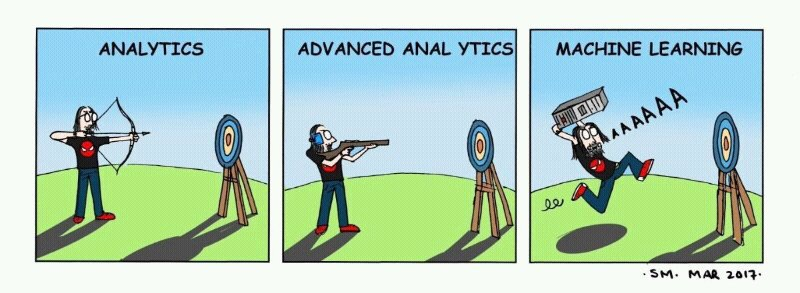
\includegraphics[width=\textwidth]{images/Chapter01_Intro/joke.jpg}
    \caption{Machine Learning.}
    \scriptsize{we could write some more}
    \label{fig: lung-breast-cancer}
    % \href{https://gco.iarc.fr}{Global cancer observatory}
\end{figure}


\section{Research Focus and Objectives}
\lipsum[2-4]
\subsection{Research question and Hypothesis}
\label{ResearchQuestion}
\lipsum[2-4]
\begin{tcolorbox}[colback=blue!5,colframe=blue!40!black,title=Hypothesis] %New Hypothesis
\textit{A hypothesis is not a question.}
\end{tcolorbox}


\subsection{Specific goals of the Research}
\label{specific-goals}
\lipsum[2-4]
\begin{enumerate}
    \item one.
    \item two.
    
\end{enumerate}

\section{Value of this Research}

\lipsum[2-4]
The remaining of this thesis is organized as follows:\\

\textbf{Chapter 1: Introduction} \\  
\lipsum[1]
 \\

\textbf{Chapter 2: Theoretical Framework }\\
\lipsum[2]
\\

\textbf{Chapter3: Research Methods} \\
\lipsum[2]\\

\textbf{Chapter4: Results} \\
\lipsum[2]\\

\textbf{Chapter 5: Conclusion} \\
\lipsum[2]\\

\textbf{Chapter 6: References} \\
\lipsum[2]
